\documentclass{beamer}
\usepackage{times}
\usepackage{tikz}
\usepackage{beamerthemesplit}
\usepackage{tcolorbox}

\title{A Tutorial of White-Box Cryptography \\ Chapter 3 Implementations}
\author{Zheng Gong\inst{1,2}\\ \url{cis.gong@gmail.com}}
\institute{\inst{1}{School of Computer Science, South China Normal University} \\ \inst{2}{Mobile Applications And Security Engineering Center of Guangdong Province}}

\date{\today}

\begin{document}

\frame
{
 \titlepage
}

\section[Outline]{}
\frame{\tableofcontents}

\section{White-box DES}
\frame
{
  \frametitle{Chow et al.'s white-box DES}

\begin{itemize}
\item At ACM DRM 2002, Chow et al. proposed a white-box DES implementation for DRM applications.
\item The terminology and notation of this implementation are inherited in the following schemes.
\item In this very beginning paper of white-box cryptography, Chow \textit{et al.} use \textit{locally secure} to illustrate the protection of key extraction with the Man-At-The-End attack.
\end{itemize}

\begin{center}
\begin{tikzpicture}
    \node[anchor=south west,inner sep=0] (image) at (0,0) { 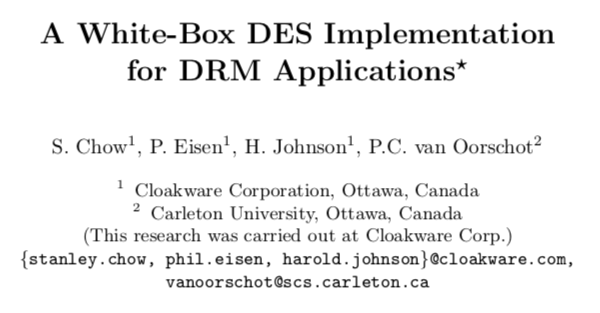
\includegraphics[width=7cm, height=3.5cm]{./pics/WBC_DES_2002.png}};

    %\begin{scope}[x={(image.south east)},y={(image.north west)}]
        %\draw[help lines,xstep=.1,ystep=.1] (0,0) grid (1,1);
        %\foreach \x in {0,1,...,9} { \node [anchor=north] at (\x/10,0) {0.\x}; }
        %\foreach \y in {0,1,...,9} { \node [anchor=east] at (0,\y/10) {0.\y}; }
        %\draw[green, ultra thick, rounded corners] (0.24,0.18) rectangle (0.50,0.32);
    %\end{scope}
\end{tikzpicture}
\end{center}
}

\subsection{Terminology and Notion}

\frame
{
\frametitle{The main concept of encoding}
For linear transformation, there are three kinds of encoding terms to obscure the intermediate values of round function.
\newline
\begin{itemize}
\item encoding

\item concatenated encoding

\item networked encoding
\end{itemize}
}

\frame
{
\frametitle{Encoding}
\begin{definition}{\textbf{(encoding)}}
Let $X$ be a transformation from $m$ to $n$ bits. Choose an $m$-bit bijection $F$ and an $n$-bit bijection $G$. Call $X^{'}=G \circ X \circ F^{-1}$ an encoded version of $X$. $F$ is an input encoding and G is an output encoding.
\end{definition}
}

\frame
{
\frametitle{Concatenated encoding}
\begin{definition}{\textbf{(concatenated encoding)}}
Consider bijection $F_{i}$ of size $n_{i}$, where $n_{1} + n_{2} + \cdots + n_{k}=n$. Let $||$ denote vector concatenation.
The function concatenation $F_{1}||F_{2}||\cdots||F_{k}$ is the bijection F such that, for any $n$-bit vector $b = (b_{1}, b_{2}, \cdots, b_{n})$, $F(b) = F_{1}(b_{1}, \cdots, b_{n_{1}})||F_{2}(b_{n_{1}+1}, \cdots, b_{n_{1}+n_{2}})||\cdots||F_{k}(b_{n+1}+\cdots+n_{k-1}, \cdots, b_{n})$. For such a bijection $F$, plainly $F^{-1} = F^{-1}_{1}||F^{-1}_{2}||\cdots||F^{-1}_{k}$.
\end{definition}

}

\frame
{
\frametitle{Networked encoding}
\begin{definition}{\textbf{networked encoding}}
A network encoding for computing $Y \circ X$ (i.e., transformation $X$ followed by transformation $Y$) is an encoding of the form:
\[Y^{'} \circ X^{'} = (H \circ Y \circ G^{-1}) \circ (G \circ X \circ F^{-1}) = H \circ (Y \circ X) \circ F^{-1}.\]
\end{definition}

}

\frame
{
\frametitle{Entropy-transference function}
$^{n}_{m}E$ is an \textit{entropy-transference function} such that $^{n}_{m}E$ maps $m$-bit vectors to $n$-bit vectors, when $m \leq n$ the mapping loses no bits of information, $m > n$ it loses at most $n-m$ bits.
}

\frame
{
\frametitle{affine transformation (\textbf{AT}) function}
A vector to vector transformation function $P$ which can be define for all $_{m}e$ by \[^{n}_{m}P(_{m}e)= ^{n}_{m}M_{m}\cdot e + _{n}d\], or \[P(e)=M\cdot e + d,\]
where $M$ is a constant matrix and $d$ is a constant \textit{displacement/masking/affine} vector.

We consider \textbf{ATs} over $GF(2)$. Note if $A$ and $B$ are \textbf{ATs}, so $A||B$ and $A \circ B$.
}

\frame
{
\frametitle{White-box precomputation}
\begin{itemize}
\item In the black-box model, a cryptographic function is algorithmically implemented beforehand and waits for inputs.

\item In the white-box model, the secret key is known first by the white-box tables generator (it might not be needed as server).
\end{itemize}

Two transformations are required for the white-box cryptosystems:
\begin{enumerate}
\item the white-box algorithm: transform the black-box version of algorithm into white-box version
\begin{itemize}
\item affine transformation
\item encoding
\end{itemize}
\item the white-box key tables: transform the round keys into a series of white-box key tables.
\end{enumerate}
}

\subsection{Producing encoded implementations}

\frame
{
\frametitle{Mixing bijection}
A \textit{mixing bijection} is a bijective \textbf{AT} which attempts to maximize the dependency of each output bit on all input bits.

\begin{itemize}
\item For example, a bit permutation layer $P$ might be sparse in a matrix representation (such as the $P$ layer in DES).

\item In order to diffuse more information over more bits, we can represent such a permutation $P=J \circ K$, where $J = P \circ K^{-1}$.
\end{itemize}
}

\frame
{
\frametitle{I/O-blocked encoding}
An arbitrary function $^{n}_{m}P$, where $m$ and $n$ are large, cannot simply be encoded using two arbitrary bijective encodings as $P'=G\circ P \circ F^{-1}$ using a look-up table. \newline

For example, a transformation $^{8}_{16}P$ requires $2^{8}\times 16=2^{12}$ bits (4Kb) storage, whilst $^{16}_{64}P$ requires $2^{16} \times 32=2^{21}$ bits (2Mb!).\newline

\textbf{Solution:}
\begin{itemize}
\item Let $F_{P} = (F_{1}||F_{2}||\cdots||F{j}) \circ J$ and $G_{P}=(G_{1}||G_{2}||\cdots||G_{k})\circ K$.
\item Concatenated encoding: $F_{j}$ is $^{a}_{a}F$ and $G_{k}$. is $^{b}_{b}G$.
\item $P'=G_{P}\circ P \circ F_{P}^{-1}$.
\end{itemize}
}

\frame
{
\frametitle{Combined function encoding}
For functions $P$ and $Q$ that happened to be evaluated  together, we could choose an encoding $P||Q$ such as $G\circ (P||Q) \circ F^{-1}$.\newline

For two $4$-bit sboxes $S_{1}(_{4}e)$ and $S_{2}(_{4}e)$, we can combine them together as an $8$-bit sbox $(S_{1}||S_{2})(_{8}e)$.

}

\frame
{
\frametitle{By-pass encoding}
In general, we want the implementation of each transform to have extra entropy at both the input and output, so that it is more difficult to extract the core.\newline

For a function $^{n}_{m}P$, we can put a \textit{by-pass encoding} $^{b}_{a}E$ such that $^{n+b}_{m+a}P'=G\circ (P||^{b}_{a}E)\circ F^{-1}$.
}

\frame
{
\frametitle{Split-path encoding}
Form a function $^{n}_{m}P$, we may use an encoding that is really a concatenation of two separate encodings. That is, we define
\[^{n+k}_{m}Q(_{m}e)=P(_{m}e)||^{k}_{m}R(_{m}e)\]
The effect is that if $P$ is lossy, $Q$ may lose less information (or no information). This method is used to achieve \textit{local security}.
}

\frame
{
\frametitle{Output splitting?}
We can encode a function $P$ as $k \geq 2$ functions $P_{1}, P_{2}, \cdots, P_{k}$, where the encoded implementation for each part can mix in additional entropy. For example, \[^{n}_{m}P_{2}(_{m}e) =P(_{m}e) \oplus P_{1}(_{m}e)\]

}

\subsection{Wide-input encoded ATs}

\frame
{
\frametitle{Wide-input encoding}
\begin{itemize}
\item Due to the storage costs, it is impractical to improve the input-size of an sbox.

\item But we can use a concatenated encoding, build a wide-input encoding for a network of sboxes.
\end{itemize}

For an sbox $S$ with $n$-bit input and output (normally 4-bit or 8-bit), we can use the following wide-input encoding method:
\[^{k\times n}_{k\times m}A \circ (S_{1}||S_{2}||\cdots||S_{k})= ^{n}_{m}A_{1} \circ S_{1}||^{n}_{m}A_{2} \circ S_{2}||\cdots||^{n}_{m}A_{k} \circ S_{k}\]
}

\frame
{
\frametitle{First step of Chow et al.'s white-box DES in two rounds}
\begin{center}
\begin{tikzpicture}
    \node[anchor=south west,inner sep=0] (image) at (0,0) { 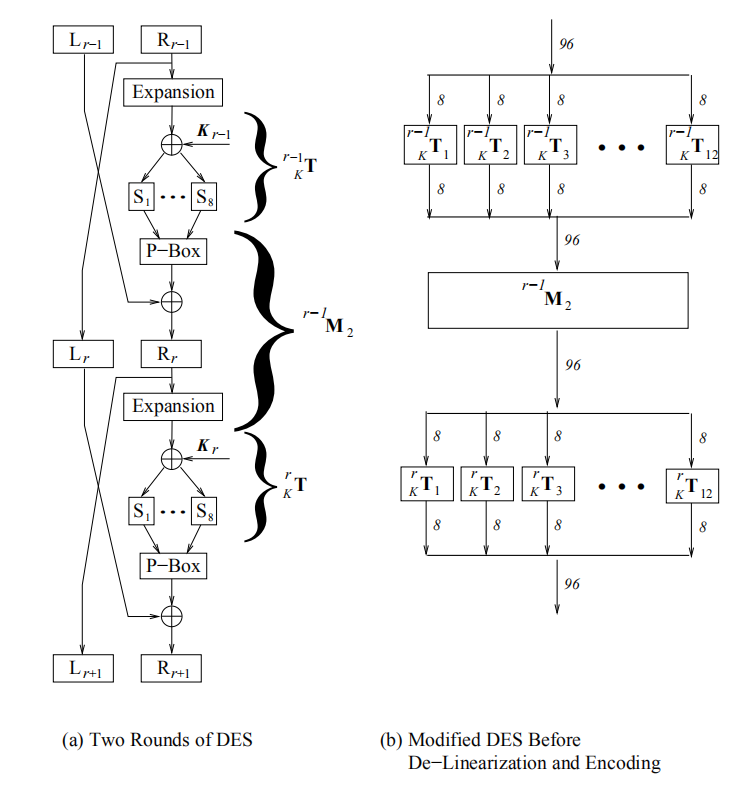
\includegraphics[width=7cm, height=7cm]{./pics/TwoRound_WBDES.png}};

    %\begin{scope}[x={(image.south east)},y={(image.north west)}]
        %\draw[help lines,xstep=.1,ystep=.1] (0,0) grid (1,1);
        %\foreach \x in {0,1,...,9} { \node [anchor=north] at (\x/10,0) {0.\x}; }
        %\foreach \y in {0,1,...,9} { \node [anchor=east] at (0,\y/10) {0.\y}; }
        %\draw[green, ultra thick, rounded corners] (0.24,0.18) rectangle (0.50,0.32);
    %\end{scope}
\end{tikzpicture}
\end{center}
}

\frame
{
\frametitle{DES sbox and its local security}
Let $6$-bit input $a=a_{0}a_{1}\cdots a_{5}$ and DES $6$-bit input and $4$-bit output sbox $^{6}_{4}S(.)$. To build a local secure look-up table $T$, we have
\[^{8}_{8}T(a||^{2}b)=^{6}_{4}S(a)||a_{0}||a_{5}||b.\]

\begin{tikzpicture}
    \node[anchor=south west,inner sep=0] (image) at (0,0) { 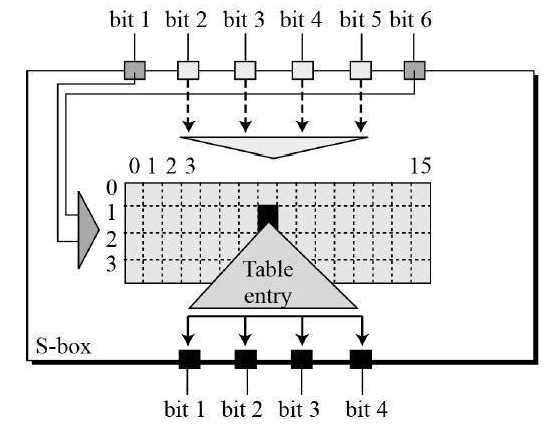
\includegraphics[width=5cm, height=5cm]{./pics/DES_Sbox.png}};
    
     \node[anchor=south west,inner sep=0] (image) at (0,0) { 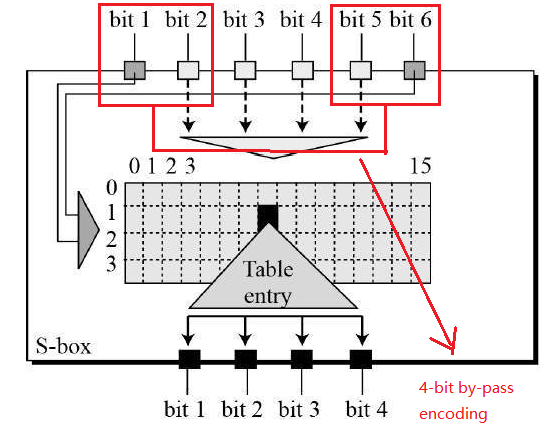
\includegraphics[width=5cm, height=5cm]{./pics/WBDES_Tbox.png}};

    %\begin{scope}[x={(image.south east)},y={(image.north west)}]
        %\draw[help lines,xstep=.1,ystep=.1] (0,0) grid (1,1);
        %\foreach \x in {0,1,...,9} { \node [anchor=north] at (\x/10,0) {0.\x}; }
        %\foreach \y in {0,1,...,9} { \node [anchor=east] at (0,\y/10) {0.\y}; }
        %\draw[green, ultra thick, rounded corners] (0.24,0.18) rectangle (0.50,0.32);
    %\end{scope}
\end{tikzpicture}



}

\section{White-box AES}

\frame
{
\frametitle{Chow et al.'s white-box AES}


\begin{tikzpicture}
    \node[anchor=south west,inner sep=0] (image) at (0,0) { 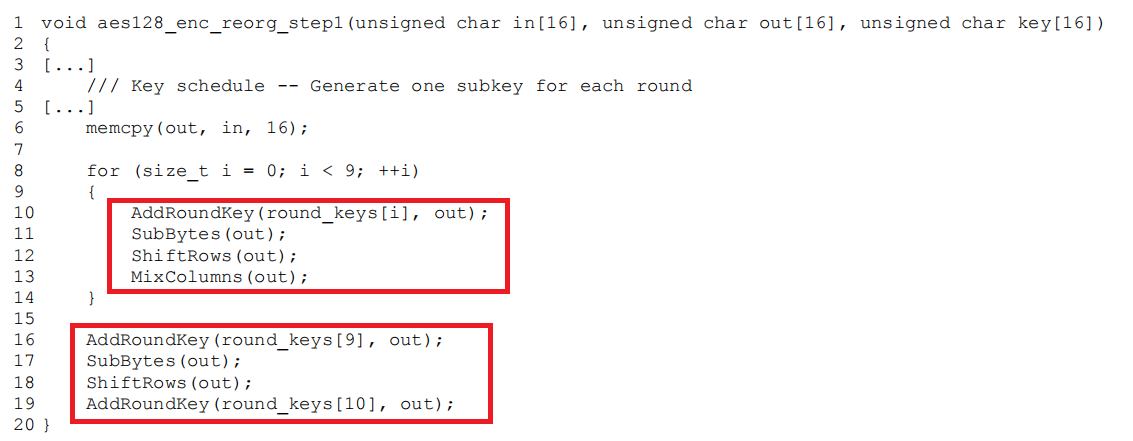
\includegraphics[width=7cm, height=3cm]{./pics/AES.png}};

    %\begin{scope}[x={(image.south east)},y={(image.north west)}]
        %\draw[help lines,xstep=.1,ystep=.1] (0,0) grid (1,1);
        %\foreach \x in {0,1,...,9} { \node [anchor=north] at (\x/10,0) {0.\x}; }
        %\foreach \y in {0,1,...,9} { \node [anchor=east] at (0,\y/10) {0.\y}; }
        %\draw[green, ultra thick, rounded corners] (0.24,0.18) rectangle (0.50,0.32);
    %\end{scope}
\end{tikzpicture}


\begin{tikzpicture}
    \node[anchor=south west,inner sep=0] (image) at (0,0) { 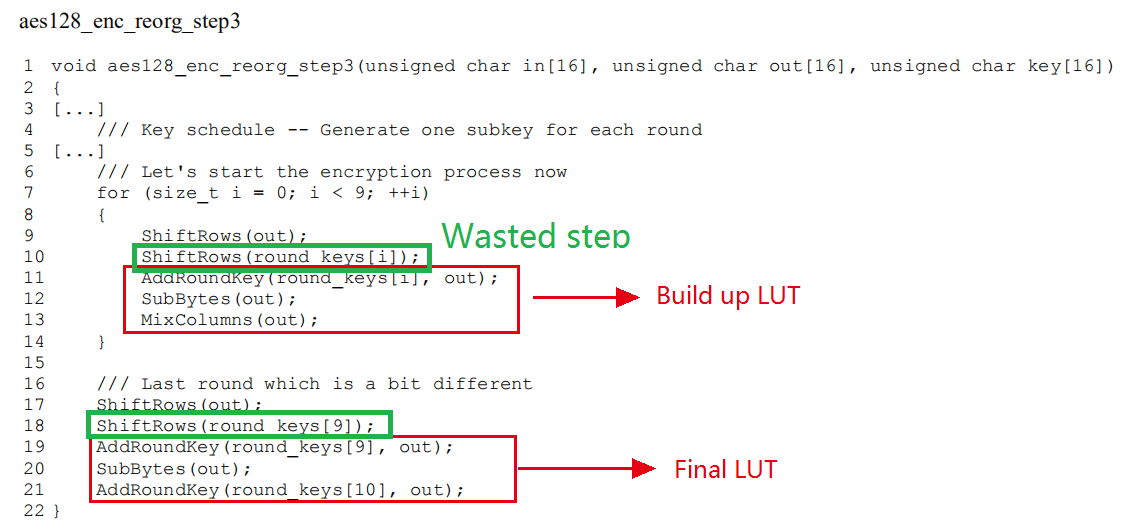
\includegraphics[width=7cm, height=3cm]{./pics/Chow_WBAES.png}};

    %\begin{scope}[x={(image.south east)},y={(image.north west)}]
        %\draw[help lines,xstep=.1,ystep=.1] (0,0) grid (1,1);
        %\foreach \x in {0,1,...,9} { \node [anchor=north] at (\x/10,0) {0.\x}; }
        %\foreach \y in {0,1,...,9} { \node [anchor=east] at (0,\y/10) {0.\y}; }
        %\draw[green, ultra thick, rounded corners] (0.24,0.18) rectangle (0.50,0.32);
    %\end{scope}
\end{tikzpicture}


}


\frame
{
\begin{center}
\textbf{Thanks for your attentions!}
\end{center}
\begin{center}
\begin{tikzpicture}
    \node[anchor=south west,inner sep=0] (image) at (0,0) { 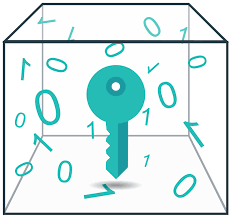
\includegraphics[width=4cm, height=4cm]{./pics/WBC_BG.png}};

    %\begin{scope}[x={(image.south east)},y={(image.north west)}]
        %\draw[help lines,xstep=.1,ystep=.1] (0,0) grid (1,1);
        %\foreach \x in {0,1,...,9} { \node [anchor=north] at (\x/10,0) {0.\x}; }
        %\foreach \y in {0,1,...,9} { \node [anchor=east] at (0,\y/10) {0.\y}; }
        %\draw[green, ultra thick, rounded corners] (0.24,0.18) rectangle (0.50,0.32);
    %\end{scope}
\end{tikzpicture}

\end{center}
}

\end{document}
